TODO: Rewrite/Adapt/Remove this paragraph now that it's been integrated

What do they look like

include theoretical example

several concrete examples (codingsepctator, Sando, Eclipse study)

%Software systems often keep a record about what event was completed (or not) in the form of a log file. The information collected in the log file is often used for diagnostic purposes. If a system failure occurs, the logs for that period can be inspected to see which sequence of events were executed by the system and what were the values for the dynamic information in those events. Each log line can be traced back to a particular line of code where the method to log this information was called. Hene, we can get complete information on what events were executed. The log message store information about the branches taken by that particular instance of execution and the values for variables in the code. Due to these reasons, the information in the log file is collected as a serially ordered flat text file. In short, a log file is a collection of log lines, with each of them having information about a single event, its time of execution and the dynamic information about variable values. Note that each log line may span across multiple lines, but provides information to distinct two adjacent log lines.



\begin{figure*}[t]
 \centering
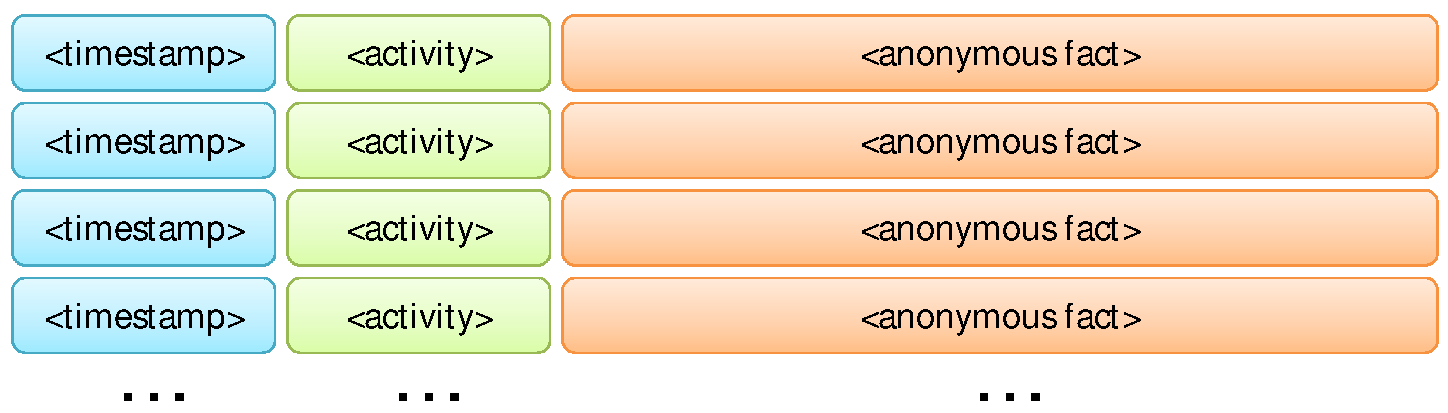
\includegraphics[width=1\columnwidth]{../Graphics/activityLogTheoretical.pdf}
%\caption{Pairwise matches across categories, including matching and mismatching pairs.}
\label{fig:theoretical}
\end{figure*}



\begin{figure*}[t]
 \centering
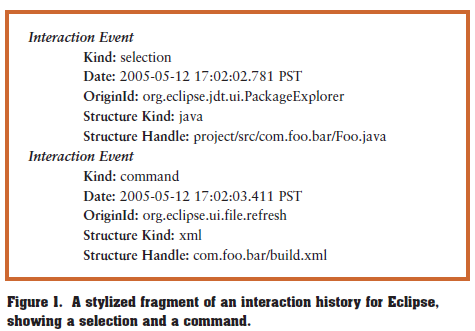
\includegraphics[width=0.5\columnwidth]{AnalyzingUsageData/activityEvent}
\caption{Activities as Captured in an Eclipse Usage Data Study}
\label{fig:activity}
\end{figure*}

\begin{figure*}[t]
 \centering
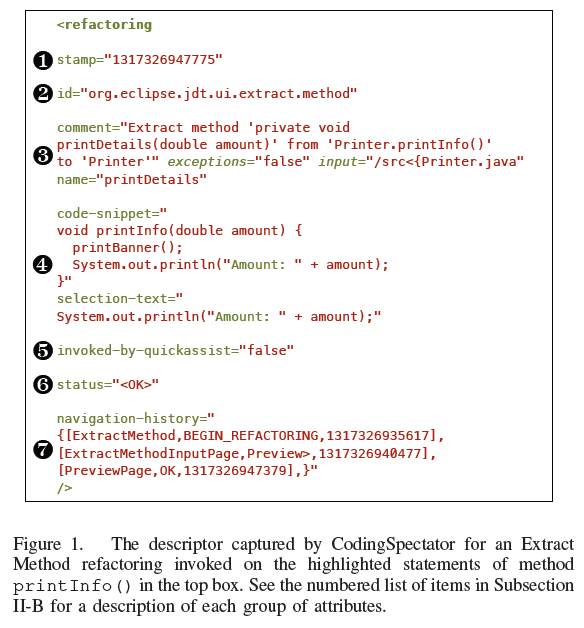
\includegraphics[width=0.5\columnwidth]{AnalyzingUsageData/codingSpectator}
\caption{Activities as Captured in a CodingSpectator Study of Refactoring Events}
\label{fig:activit}
\end{figure*}

